\documentclass[10pt,aspectratio=169]{beamer}

\usetheme{Madrid}
\usecolortheme{whale}

% Custom colors
\definecolor{mainblue}{HTML}{004983}
\definecolor{darkblue}{HTML}{002F5F}
\definecolor{accentblue}{HTML}{4682B4}
\definecolor{lightgray}{HTML}{F0F0F0}

\setbeamercolor{structure}{fg=mainblue}
\setbeamercolor{title}{fg=white,bg=mainblue}
\setbeamercolor{frametitle}{fg=white,bg=mainblue}
\setbeamercolor{block title}{fg=white,bg=mainblue}
\setbeamercolor{block body}{bg=lightgray}

\usepackage{amsmath,amssymb,bm}
\usepackage{graphicx}
\usepackage{tikz}
\usetikzlibrary{arrows.meta,positioning,calc,decorations.pathmorphing,shapes.geometric}

\graphicspath{{pics/}}

\title[FFO-CO \& Frustrated Spins]{Function-Free Optimization via Comparison Oracles\\[4pt]
{\small A Hypothetical Strategy for Frustrated Spin Systems}}
\author{Learning Notes on arXiv 2604.26867v2}
\date{\today}

\begin{document}

% ============================================================
% Title
% ============================================================
\begin{frame}
  \titlepage
\end{frame}

% ============================================================
% Frame 1: Geometric Frustration — Kagome & Pyrochlore
% ============================================================
\begin{frame}{Frustrated Spin Systems: Geometric Frustration}
\begin{columns}[T]
\begin{column}{0.48\textwidth}
  \centering
  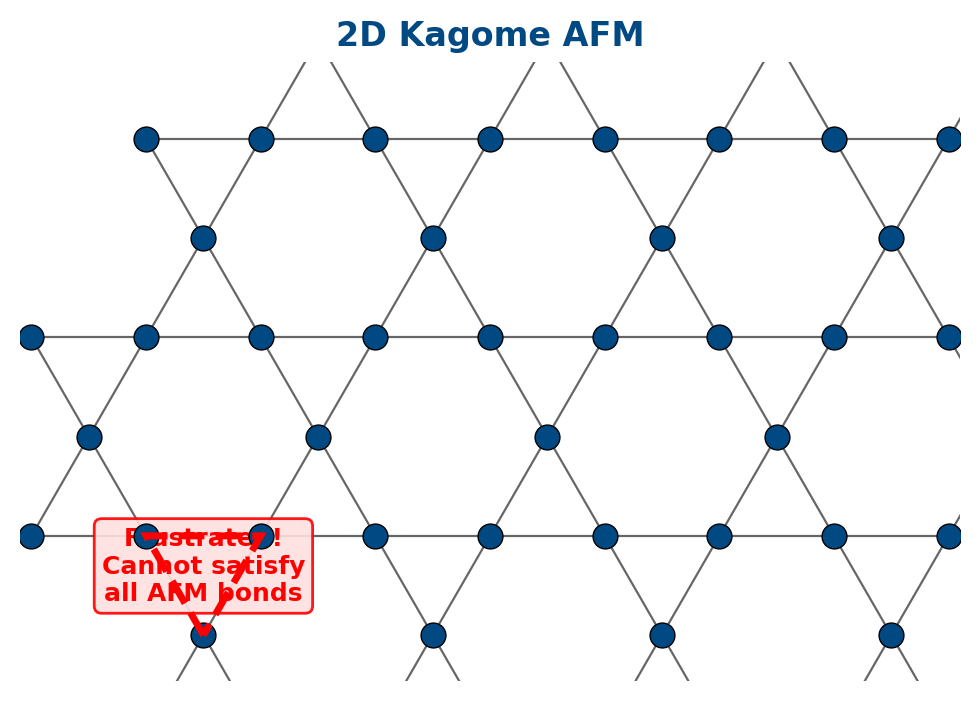
\includegraphics[width=0.75\linewidth]{kagome_afm.png}\\[2pt]
  \textbf{2D Kagome AFM}\\[1pt]
  \small $H = J\sum_{\langle ij\rangle}\bm{S}_i\cdot\bm{S}_j,\; J>0$\\
  Cannot satisfy all 3 AFM bonds on a triangle\\[4pt]
  \footnotesize\color{mainblue}
  Geometric frustration $\Rightarrow$ exponentially many
  near-degenerate minima $\Rightarrow$ \textbf{rugged energy landscape}
\end{column}
\begin{column}{0.48\textwidth}
  \centering
  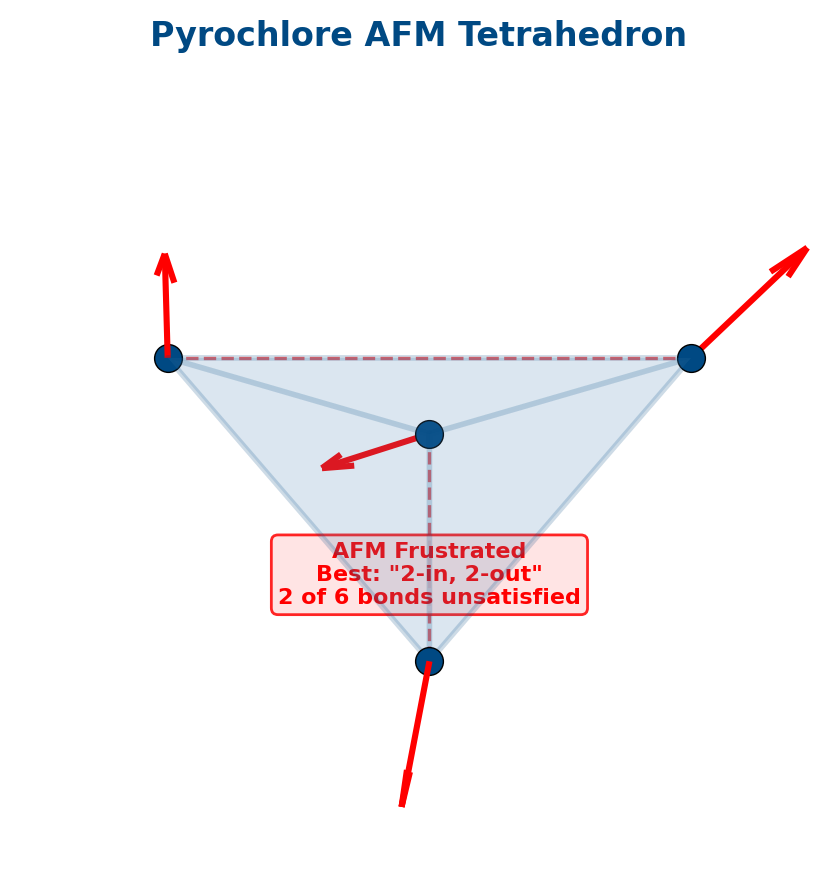
\includegraphics[width=0.75\linewidth]{pyrochlore_frust.png}\\[2pt]
  \textbf{3D Pyrochlore AFM}\\[1pt]
  \small Corner-sharing tetrahedra\\
  Best: ``2-in, 2-out'' $\Rightarrow$ 2/6 bonds unsatisfied
\end{column}
\end{columns}
\end{frame}

% ============================================================
% Frame 2: Heisenberg — Continuous S² Parameter Space
% ============================================================
\begin{frame}{Heisenberg Model: Continuous $S^2$ Configuration Space}
\begin{columns}[T]
\begin{column}{0.55\textwidth}
  \begin{itemize}
    \item Heisenberg spin: $\bm{S}_i \in S^2$ (unit sphere)
    \item Configuration space: $(S^2)^N$
    \item Parameterize via spherical coordinates:
      \[
        \bm{S}_i = (\sin\theta_i\cos\varphi_i,\;
                     \sin\theta_i\sin\varphi_i,\;
                     \cos\theta_i)
      \]
    \item Maps $(S^2)^N \to \mathbb{R}^{2N}$ via $(\theta_i,\varphi_i)$
    \item \textbf{Frustration}: competing interactions demand
          mutually contradictory spin orientations
    \item Coordinate singularities at $\theta=0,\pi$
  \end{itemize}
\end{column}
\begin{column}{0.42\textwidth}
  \centering
  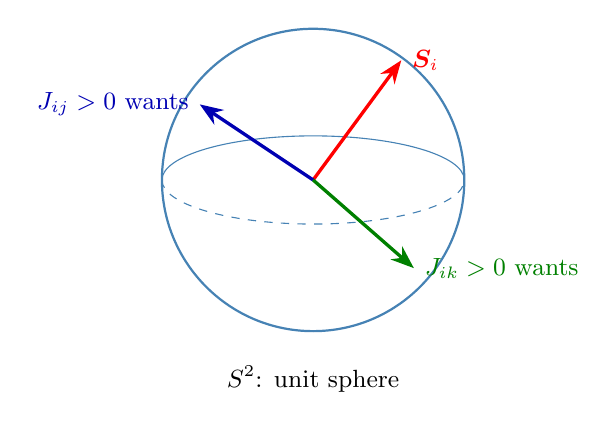
\begin{tikzpicture}[scale=1.6]
    % Unit sphere (circle in 2D projection)
    \draw[accentblue,thick] (0,0) circle (1.2);
    \draw[accentblue,dashed] (-1.2,0) arc (180:360:1.2 and 0.35);
    \draw[accentblue] (-1.2,0) arc (180:0:1.2 and 0.35);

    % Three competing arrows
    \draw[-{Stealth},red,very thick] (0,0) -- (0.7,0.95)
      node[right]{\small $\bm{S}_i$};
    \draw[-{Stealth},blue!70!black,very thick] (0,0) -- (-0.9,0.6)
      node[left]{\small $J_{ij}>0$ wants};
    \draw[-{Stealth},green!50!black,very thick] (0,0) -- (0.8,-0.7)
      node[right]{\small $J_{ik}>0$ wants};

    % Labels
    \node[below] at (0,-1.4) {\small $S^2$: unit sphere};
  \end{tikzpicture}
\end{column}
\end{columns}

\vspace{4pt}
\begin{block}{Connection to FFO-CO}
Continuous parameter space $\mathbb{R}^{2N}$ is a prerequisite for FFO-CO.\\
But frustrated systems violate \emph{convex preference} $\Rightarrow$ non-trivial extension required.
\end{block}
\end{frame}

% ============================================================
% Frame 3: Edwards-Anderson Random Bond Model
% ============================================================
\begin{frame}{Edwards--Anderson Model: Quenched Random Couplings}
\begin{columns}[T]
\begin{column}{0.50\textwidth}
  \centering
  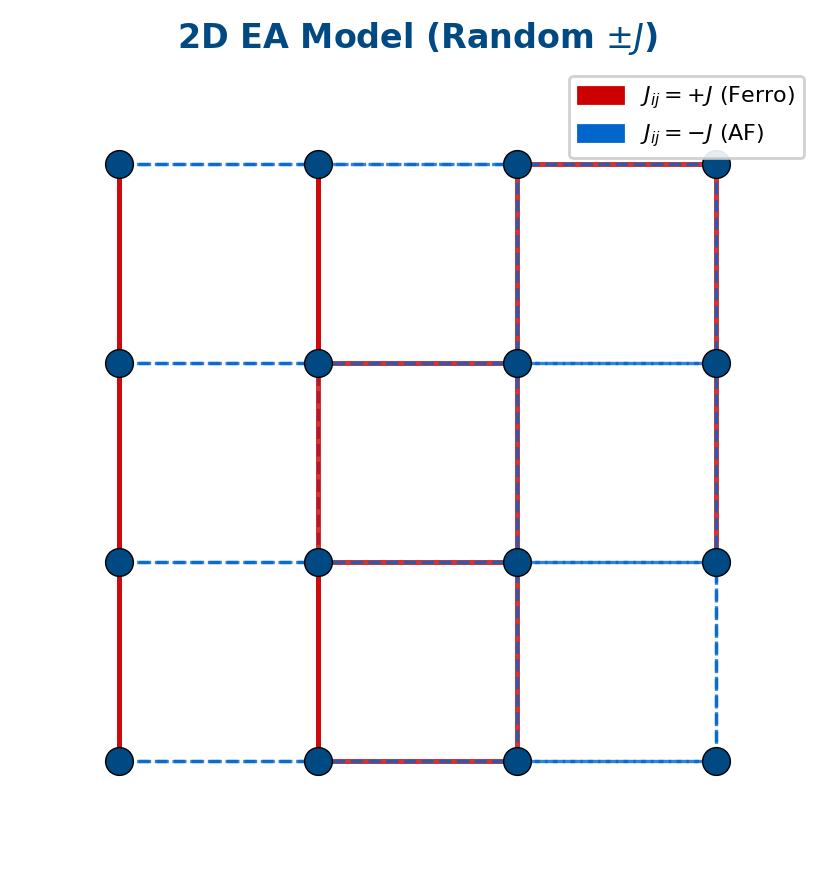
\includegraphics[width=0.85\linewidth]{ea_random.png}
\end{column}
\begin{column}{0.48\textwidth}
  \begin{itemize}
    \item Hamiltonian:
      \[
        H = -\sum_{\langle ij\rangle} J_{ij}\,\bm{S}_i\cdot\bm{S}_j
      \]
    \item $J_{ij}$ quenched random: $\pm J$ (bimodal) or $\mathcal{N}(0,\sigma^2)$ (Gaussian)
    \item \textbf{Rugged landscape}: $\sim e^{cN}$ local minima
    \item Finding ground state: \textbf{NP-hard}
    \item Prototype of \emph{spin glass} physics
  \end{itemize}
\end{column}
\end{columns}
\end{frame}

% ============================================================
% Frame 4: FFO-CO Strategy on Rugged Landscape (core)
% ============================================================
\begin{frame}{A Hypothetical FFO-CO Strategy for Rugged Landscapes}
\centering
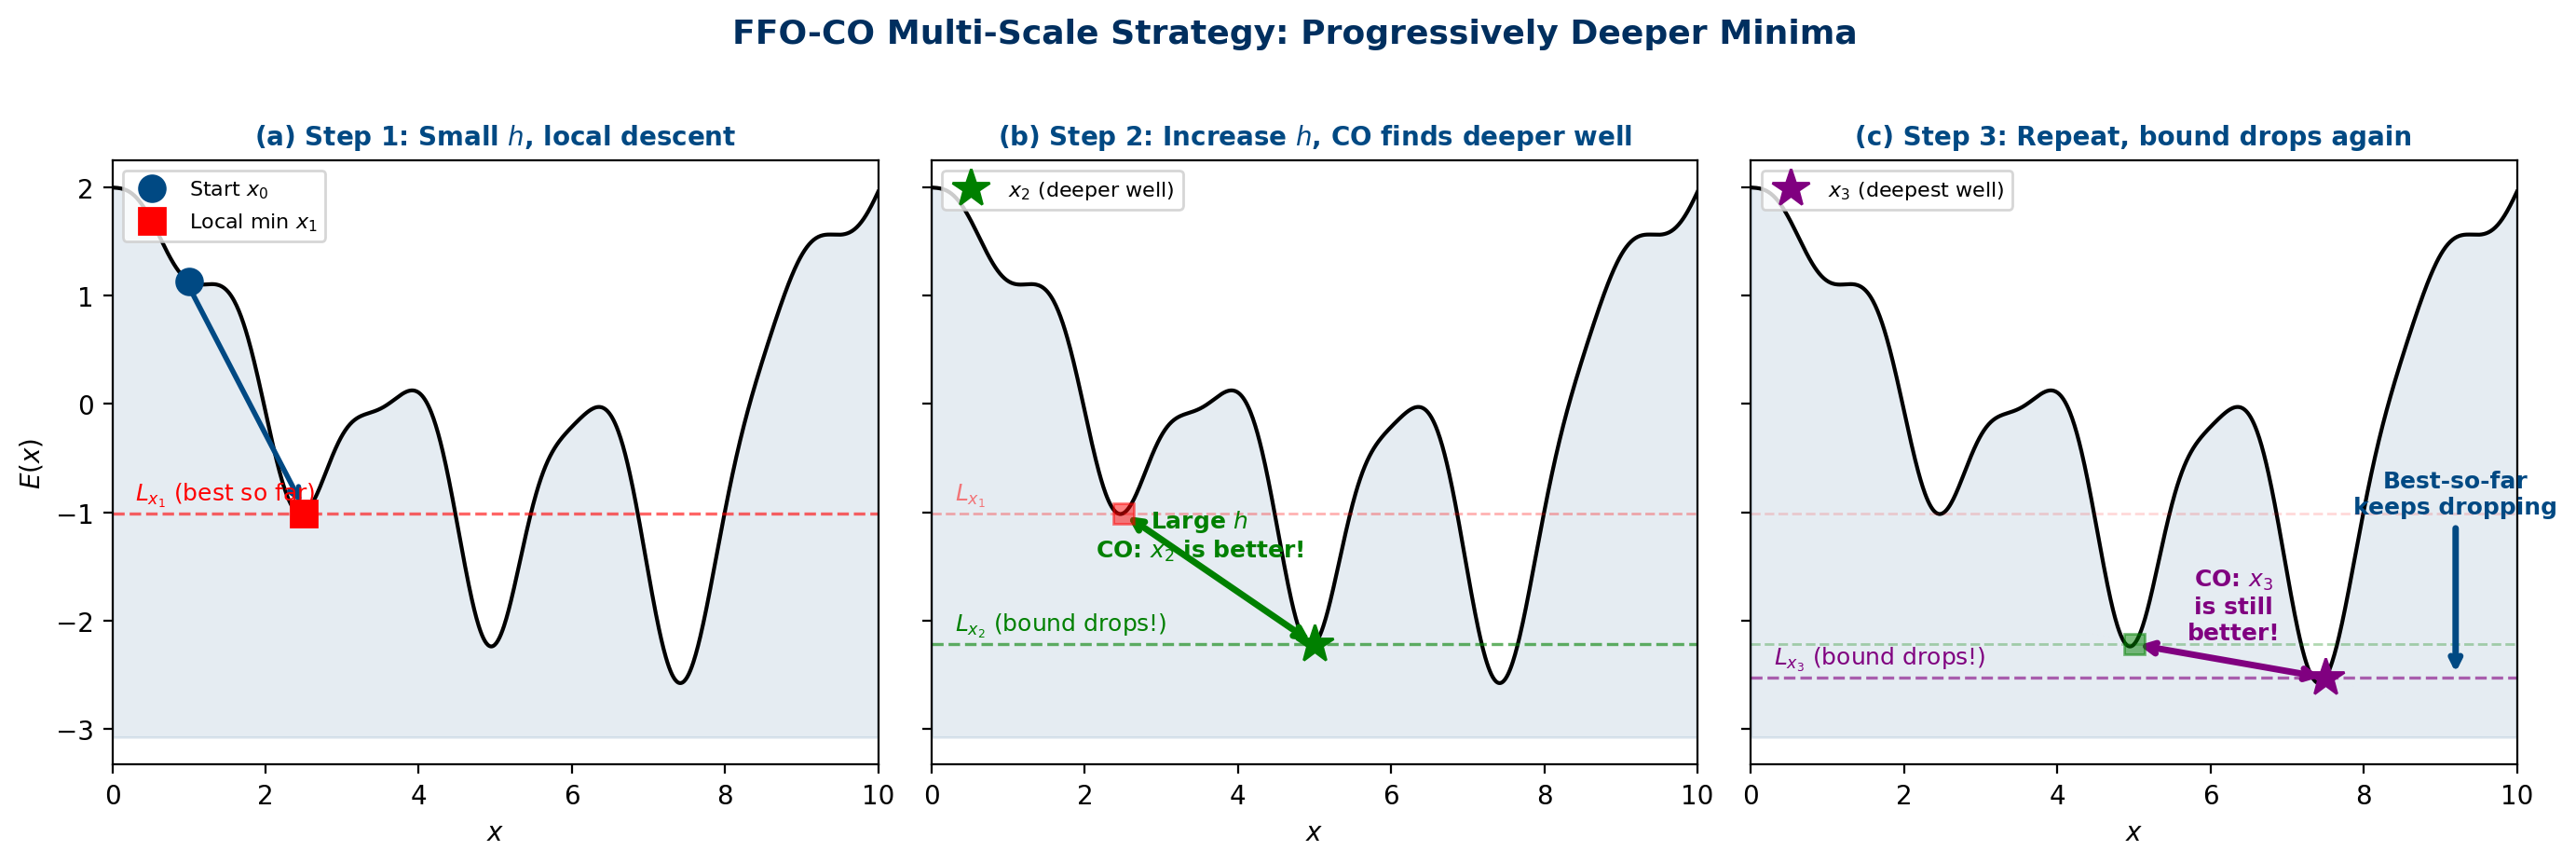
\includegraphics[width=0.95\linewidth]{rugged_ffo_co.png}

\vspace{4pt}
\begin{enumerate}
  \item \textbf{Small $h$}: FFO-CO local descent $\to$ local minimum $x_1$
  \item \textbf{Increase $h$}: comparison oracle discovers a \emph{better} (deeper) region
        $\Rightarrow$ level set $L_{x_2}$ drops below $L_{x_1}$
  \item \textbf{Small $h$} in new region $\to$ local min $x_2$; repeat
        $\Rightarrow$ best-so-far bound keeps dropping
\end{enumerate}

\vspace{2pt}
\small
\textbf{Key insight}: Comparison inconsistency (same direction, different $h$
$\Rightarrow$ flipped result) exposes \emph{separated level sets} — structural
information that gradients cannot provide.
\end{frame}

% ============================================================
% Frame 5: VMC Application Scenario
% ============================================================
\begin{frame}{VMC: Application Scenario for FFO-CO}
\begin{columns}[T]
\begin{column}{0.52\textwidth}
  \begin{block}{VMC Pipeline}
  \centering
  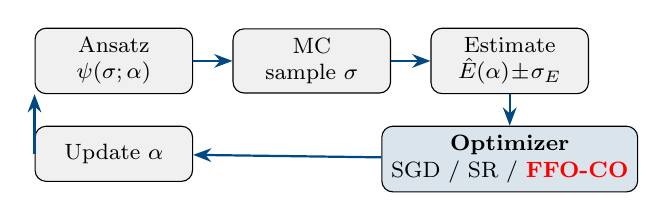
\begin{tikzpicture}[
    box/.style={draw,rounded corners,fill=lightgray,minimum height=0.7cm,
                minimum width=2.0cm,font=\footnotesize,align=center},
    arr/.style={-{Stealth},thick,mainblue},
    node distance=0.5cm
  ]
    \node[box] (ansatz) {Ansatz\\$\psi(\sigma;\alpha)$};
    \node[box,right=of ansatz] (mc) {MC\\sample $\sigma$};
    \node[box,right=of mc] (est) {Estimate\\$\hat{E}(\alpha)\!\pm\!\sigma_E$};
    \node[box,below=0.4cm of est,fill=mainblue!15] (opt)
      {\textbf{Optimizer}\\SGD / SR / \textcolor{red}{\textbf{FFO-CO}}};
    \node[box,below=0.4cm of ansatz] (upd) {Update $\alpha$};
    \draw[arr] (ansatz) -- (mc);
    \draw[arr] (mc) -- (est);
    \draw[arr] (est) -- (opt);
    \draw[arr] (opt) -- (upd);
    \draw[arr] (upd.west) -| (ansatz.south west);
  \end{tikzpicture}
  \end{block}
  \vspace{2pt}
  \small
  \begin{itemize}
    \item Variational: $E(\alpha)=\frac{\langle\psi|H|\psi\rangle}{\langle\psi|\psi\rangle}\geq E_0$
    \item Jastrow: $\psi=\exp\!\bigl(\sum_{i<j}\alpha_{ij}\,\sigma_i\sigma_j\bigr)$
    \item MC noise: $\sigma_E \propto 1/\!\sqrt{N_s}$
  \end{itemize}
\end{column}
\begin{column}{0.46\textwidth}
  \begin{block}{Noise: Gradient vs Sign}
  \small
  \begin{tabular}{@{}lcc@{}}
    & SGD/SR & FFO-CO \\
    \hline
    Needs & $\nabla E$ & $\operatorname{sign}(\Delta E)$\\[2pt]
    Noise & $\frac{\sigma_E}{h}$ \textcolor{red}{$\uparrow$}
          & $P_{\mathrm{ok}}>97\%$\\
          & (amplified) & ($|\Delta E|>3\sigma$)\\[2pt]
    Signal & $|\partial E/\partial\alpha|$ & $|\Delta E|$ \\
           & (fixed) & (\textcolor{mainblue}{tunable via $h$})\\
  \end{tabular}
  \end{block}
  \vspace{4pt}
  \footnotesize
  \textbf{Key}: sign signal can be amplified by
  increasing comparison radius~$h$;\\
  gradient signal is fixed and its estimation
  requires dividing by~$h$.
\end{column}
\end{columns}

\vspace{4pt}
\begin{block}{}
\centering\small
FFO-CO replaces only the \textbf{optimizer} — ansatz, sampler, $E_{\mathrm{loc}}$ computation are fully reused.
\end{block}
\end{frame}

% ============================================================
% Frame 6: Key Observations & Open Questions
% ============================================================
\begin{frame}{Key Observations \& Open Questions}
\begin{columns}[T]
\begin{column}{0.48\textwidth}
  \begin{block}{Comparison Oracle vs Gradient}
    \begin{itemize}
      \item CO gives \textbf{global level-set ranking}\\
            between distant points
      \item Gradient is \emph{purely local}\\
            — no relationship between distant gradients
      \item In noisy settings:\\
            $\operatorname{sign}(\Delta E)$ more robust\\
            than $|\nabla E|$
    \end{itemize}
  \end{block}
\end{column}
\begin{column}{0.48\textwidth}
  \begin{block}{Comparison Consistency\\= Non-convexity Detector}
    \begin{itemize}
      \item Same direction, different $h$:\\
            flipped comparison $\Rightarrow$ non-convexity
      \item Binary search oscillation\\
            $\Rightarrow$ level-set self-intersection
      \item Multi-direction contradictions\\
            $\Rightarrow$ multi-basin structure
    \end{itemize}
  \end{block}
\end{column}
\end{columns}

\vspace{4pt}
\begin{alertblock}{Core Argument}
``More information $\neq$ better performance'' — when gradient magnitude
is unreliable (VMC, DMFT), using only \emph{ordinal}
information with adaptive $h$ may outperform Adam-like GD variants.
\end{alertblock}

\vspace{2pt}
\footnotesize Ref: K.\ Scheinberg \& Z.\ Xiong, arXiv:2604.26867v2 (2026).
\end{frame}

\end{document}
